% main.tex -- IEEE conference paper (IEEEtran). Overleaf-ready: upload main.tex, references.bib and figs/*.png.
% Revised after the 08 critique (see REVISION_LOG.md). Every number is traced in numbers_trace.md.
% 2026-11-03: all PENDING-COLAB items resolved from the 2026-10-22 Colab ingest (see PENDING.md, numbers_trace.md). Submitted interim version: main_submitted_final_backup.tex.
\documentclass[conference]{IEEEtran}
\usepackage{cite}
\usepackage{iftex}
\ifXeTeX\usepackage{fontspec}\setmainfont{texgyretermes}[Extension=.otf,UprightFont=*-regular,BoldFont=*-bold,ItalicFont=*-italic,BoldItalicFont=*-bolditalic]\fi % local XeTeX preview only; pdfLaTeX (Overleaf) uses IEEEtran's Times
\usepackage{array}
\usepackage{amsmath,amssymb}
\usepackage{graphicx}
\usepackage{booktabs}
\usepackage{url}
\usepackage[hidelinks]{hyperref}
\graphicspath{{figs/}}
\newcommand{\B}{\textsc{B}}
\newcommand{\Dn}{\textsc{D}}
\newcommand{\Hy}{\textsc{H}}
\newcommand{\ndcg}{nDCG@10}

\begin{document}

\title{Choose Per Collection, Not Per Query: Selecting Between Sparse, Dense and Hybrid Retrieval on BEIR}

\author{\IEEEauthorblockN{Aminah Ali}
\IEEEauthorblockA{National University of Computer and Emerging Sciences (FAST-NUCES)\\
Islamabad, Pakistan\\
i269001@isb.nu.edu.pk}}

\maketitle

\begin{abstract}
We find that the best choice between keyword search (BM25), dense (embedding-based) search and a hybrid of the two depends on the collection, not on the individual query. We test both levels of choice on eight BEIR collections with three dense models (22--110M parameters). The main tests and their pass rules were fixed before running them, and every comparison is checked with paired significance tests. Our starting idea, that BM25 does worse on collections full of specialised terms, is not supported ($\rho=+0.33$, $p=0.42$, $n=8$); with eight collections, only correlations of $|\rho|\geq0.85$ can be detected. A simple, untuned 50/50 hybrid is a safe default: with BGE-base it beats BM25 on 7 of 8 collections (pooled $+0.097$ \ndcg{}). We then try to choose a system for each query. A router that reads standard query-performance-prediction (QPP) signals never beats always using the hybrid, in any of 18 versions: macro \ndcg{} is 0.525 vs.\ 0.534 with BGE-small and 0.535 vs.\ 0.548 with BGE-base. A router that reads the query text with a small fine-tuned model does worse ($-0.022$). Three other planned methods also fail: predicting the hybrid weight per query, setting it with a cross-encoder as a teacher, and re-ranking with a cross-encoder. The reason is that the QPP signals measure how hard a query is for every system, not which system suits it. In an additional analysis that was not part of the original plan, choosing once per collection works: setting the hybrid weight from 20 labelled queries gains $+0.021$ \ndcg{} with BGE-base ($+0.013$ without Touch\'e-2020).
\end{abstract}

\begin{IEEEkeywords}
BM25, dense retrieval, hybrid retrieval, query performance prediction, retriever selection, BEIR
\end{IEEEkeywords}

\section{Introduction}
Keyword search methods such as BM25 rank documents by the query words they contain~\cite{robertson2009prf}. Such methods miss relevant documents that use different words from the query, a problem known as vocabulary mismatch~\cite{furnas1987vocabulary}. Dense retrievers compare meanings instead of words, so in principle they avoid this. Yet on new topics, BM25 often remains a strong baseline~\cite{thakur2021beir}. Interpolating dense scores with BM25 improves dense retrievers~\cite{wang2021bert}. Hybrids of the two also help on topics that the dense model was not trained on~\cite{chen2022out}. A weighted sum of the two scores is a strong way to build such a hybrid~\cite{bruch2024fusion}. Anyone setting up search for a new collection must still decide which system to use, and whether to decide once for the collection or separately for each query.

This project started from a simple idea: BM25 should do worse than dense search on collections with many specialised terms (words that are rare in everyday English). The data do not support it. Across eight BEIR collections, this ``jargon rate'' was not linked to BM25's quality in the expected direction ($\rho=+0.33$, $p=0.42$). BM25 instead did \emph{relatively} better on jargon-heavy collections ($\rho=-0.60$, $p=0.12$, for the dense gain). Inside each collection, however, BM25 did well when a query's words appeared in its relevant documents. This suggested that the query, not the topic, decides, and that a router could send each query to BM25, a dense model or the hybrid. We test that idea with tests and pass rules fixed in advance. Our contributions are:
\begin{itemize}
\item \textbf{Per-query routing does not beat a fixed hybrid.} Routers built on QPP signals do not beat a fixed, untuned hybrid in any of 18 configurations. A pre-registered router that reads the query text also fails. Three further planned methods fail as well: a per-query fusion weight, a weight set by a cross-encoder teacher, and cross-encoder re-ranking.
\item \textbf{The router learns only the collection's best system.} Even when trained on the same collection, the same signals recover only which fixed system is best for that collection. The one exception is Quora, with 8,000 training queries per fold. We also measure how much of the per-query headroom is noise.
\item \textbf{Why word overlap predicts BM25.} Of the link between word overlap and BM25 quality, 66\% is query difficulty that affects dense retrievers equally. The part that is specific to keyword matching needs relevance labels, and a version without labels carries no signal.
\item \textbf{Evidence for a simple default.} We reproduce Pyserini's flat BM25 and report effect sizes for lexical fixes, dense models and hybrids. An untuned BM25+BGE-b hybrid beats BM25 on 7 of 8 collections (pooled $+0.097$ \ndcg{}).
\end{itemize}

\section{Related Work}
\textbf{BEIR and reproducibility.} BEIR evaluates retrievers on 18 datasets without training on them, using multifield Anserini BM25 ($k_1=0.9$, $b=0.4$)~\cite{thakur2021beir}. In BEIR, BM25 followed by a cross-encoder beats BM25 on 16 of the 18 datasets, failing on ArguAna and Touch\'e-2020~\cite{thakur2021beir}. Kamalloo et al.\ provide reproducible Pyserini reference runs, including the ``flat'' (title+text) BM25 that we reproduce~\cite{kamalloo2024resources}. An earlier version of their paper names two open problems: significance testing across a heterogeneous benchmark, and shallow judgement pools that may favour lexical systems~\cite{kamalloo2024resources}. On Touch\'e-2020, neural models retrieve many short, unjudged passages; after these are removed, neural \ndcg{} improves by up to 0.52, but BM25 remains more effective~\cite{thakur2024touche}.

\textbf{Vocabulary mismatch and QPP.} Zhao and Callan diagnose term mismatch in lexical retrieval~\cite{zhao2012automatic}. Amati et al.\ expand only the queries predicted to be difficult~\cite{amati2004query}. Formal et al.\ find that neural retrievers fail to generalise term importance to new domains~\cite{formal2022match}. QPP estimates search quality without relevance labels; pre-retrieval predictors use only the query and collection statistics~\cite{hauff2008survey}. Zhao et al.\ propose pre-retrieval predictors based on query--collection similarity~\cite{zhao2008effective}. Post-retrieval predictors use the result list. Clarity compares the language of the top results with the whole collection~\cite{cronentownsend2002predicting}. WIG measures how much the top scores stand out~\cite{zhou2007query}. NQC measures the spread of the top scores~\cite{shtok2012predicting}. SMV combines score mean and spread~\cite{tao2014query}. We use the definitions collected by Meng et al.~\cite{meng2023qpp}. Faggioli et al.\ report that QPP is less accurate for neural systems and fails on the queries where lexical and neural systems disagree most~\cite{faggioli2023qpp}.

\textbf{Selecting and fusing retrievers.} Arabzadeh et al.\ fine-tune BERT classifiers to choose, per query, between sparse and dense retrieval, or between sparse retrieval and a hybrid~\cite{arabzadeh2021predicting}. Their classifiers are trained and tested within one collection, MS~MARCO, with recall@1000, and beat random assignment at equal cost~\cite{arabzadeh2021predicting}. Khramtsova et al.\ find that choosing among dense retrievers per collection without labels is ineffective on BEIR~\cite{khramtsova2023selecting}. Bruch et al.\ show that a weighted sum of scores (convex combination, CC) beats reciprocal rank fusion (RRF), and that tuning CC needs few labelled queries~\cite{bruch2024fusion}. RRF combines ranked lists by rank position~\cite{cormack2009rrf}. In legal paragraph retrieval, Mori et al.\ find that query properties change the gap between BM25 and dense models~\cite{mori2025assessing}. There, BM25 beats off-the-shelf dense models where verbatim quotes are \emph{less} common and on longer queries, while a dense model fine-tuned on that collection beats BM25 on most metrics~\cite{mori2025assessing}.

\section{Methodology}
\label{sec:method}
\subsection{Research questions and hypotheses}
We ask three questions.
\begin{itemize}
\item \textbf{RQ1 (collection level).} Does the collection's vocabulary predict when BM25 fails? Hypothesis H1 states that BM25 beats TF-IDF, which beats Boolean retrieval, on every collection. Hypothesis H2 states that BM25 gets worse as the jargon rate rises.
\item \textbf{RQ2 (query level).} Can a router that sees only the query and its result lists choose between BM25, a dense model and the hybrid better than always using the hybrid? The router hypothesis states that the router's macro \ndcg{} minus that of the always-hybrid baseline is above 0.
\item \textbf{RQ3 (explanation).} If routing fails, is the reason that the signals measure query difficulty rather than which system suits a query?
\end{itemize}
Four further tests (P1--P4) try to improve on the hybrid in other ways: P1 predicts the hybrid weight per query, P2 sets it without labels using a cross-encoder as a teacher, P3 re-ranks the hybrid with a cross-encoder, and P4 trains the router on the same collection it is tested on.

\subsection{Retrieval systems}
\begin{itemize}
\item \emph{Lexical systems}, implemented from scratch: Boolean AND/OR, TF-IDF and BM25. TF-IDF uses the SMART \texttt{ltc} weighting~\cite{salton1988term}. BM25 is Lucene-style, with $k_1=0.9$, $b=0.4$, Porter stemming and one flat title+text field. BM25 is also run with RM3 pseudo-relevance feedback~\cite{lavrenko2001relevance}. BM25 is also run with WordNet synonym expansion.
\item \emph{Dense systems}: three models. The first is all-MiniLM-L6-v2 (``MiniLM'', 22M parameters)~\cite{reimers2019sbert}. The second is bge-small-en-v1.5 (``BGE-s'', 33M parameters)~\cite{xiao2024cpack}. The third is bge-base-en-v1.5 (``BGE-b'', 110M parameters)~\cite{hf_bgebase}. Each reads at most 256 tokens and searches the whole collection exactly.
\item \emph{Hybrid}: $\Hy(\Dn)=0.5\,\mathrm{minmax}(\B)+0.5\,\mathrm{minmax}(\Dn)$ over the BM25 and dense top-1000 lists. Its weight is never tuned. RRF with $k=60$ is a secondary hybrid.
\item \emph{Re-ranker}: the cross-encoder \texttt{cross-encoder/ms-marco-MiniLM-L-6-v2} (``CE'') re-ranks a top-100 list.
\end{itemize}

\subsection{Router}
\textbf{Signals (no relevance labels).} \emph{Tier A} has 23 signals: 15 computed from the query alone (length, IDF, SCQ, VAR, avICTF, SCS, jargon and out-of-vocabulary statistics) and 8 computed from the BM25 result list (WIG, NQC, SMV, Clarity and score gaps). \emph{Tier B} adds 19 signals: the same list-based predictors on the dense list, plus measures of agreement between the BM25 and dense lists (Jaccard overlap, rank-biased overlap, cross-ranks and pseudo-coverage). Both tiers exist for all three dense models on all eight collections. For explanation only, the \emph{coverage} of a query is the mean share of its terms that occur in its relevant documents. Coverage needs labels, so it is never a router input.

\textbf{Model and decision rule.} For each query, the router predicts $\Delta_\B=\mathrm{nDCG}_\B-\mathrm{nDCG}_\Hy$ and $\Delta_\Dn=\mathrm{nDCG}_\Dn-\mathrm{nDCG}_\Hy$ with Ridge regression or gradient-boosted trees. An inner leave-one-dataset-out (LODO) loop on the training collections chooses between the two. The planned (``selected'') router picks $\arg\max\{0,\hat\Delta_\B,\hat\Delta_\Dn\}$, preferring the cheapest system ($\B<\Dn<\Hy$) within 0.005 of the maximum. Secondary variants are Ridge or trees alone, logistic classification, percentile-scaled signals, and BM25 with parameters tuned by LODO. The outer loop is LODO: train on seven collections and test on the eighth.

\textbf{Text router.} A second router reads the query text directly. It fine-tunes all-MiniLM-L6-v2 with a two-output regression head, end to end, to predict $\Delta_\B$ and $\Delta_\Dn$ from the query alone, with LODO training, Quora capped at 1,500 training queries, and no hyperparameter search. It uses the same decision rule.

\subsection{Evaluation and statistics}
The metric is \ndcg{} per query.
\begin{itemize}
\item The headline is the \emph{macro} average over collections, which gives every collection equal weight. The planned secondary measure is the \emph{micro} (query-weighted) average.
\item Per collection, we use paired randomization tests with $10^4$ sign flips~\cite{smucker2007comparison}, with Holm's correction within each planned family of tests.
\item For macro differences, we use a sign-flip test stratified by collection and a stratified percentile bootstrap 95\% confidence interval ($10^4$ resamples within collections).
\item \emph{Pooled} means a DerSimonian--Laird random-effects estimate~\cite{dersimonian1986meta}. With 5--8 collections these intervals are too narrow, so we treat the macro bootstrap as primary.
\item All random steps use seed 42.
\end{itemize}

\subsection{Planned tests and leakage control}
\begin{itemize}
\item H1 and H2 were fixed, with decision rules, in the first-phase analysis code; H2 is the question of the original project proposal.
\item The router hypothesis, the headline variant and the test families were written into an experiment log before any router result was computed.
\item P1--P4 were also fixed in advance. A result counts as an improvement only if the Holm-adjusted one-sided $p<0.05$ \emph{and} the macro gain is at least $+0.005$.
\item These logs are local files with no external timestamp.
\item The text-router test, its settings and its pass rule (macro gain $\geq+0.005$ and one-sided $p<0.05$ with BGE-b) were uploaded to a third-party service (Google Drive), which records the upload time, before any data were downloaded.
\item Results that were not planned in advance are reported separately, in Section~\ref{sec:additional}.
\item Leakage control: signal files are checked by script to contain no label-derived columns; scalers and models are fitted on training collections only; tuned BM25 parameters are chosen by LODO; the cross-encoder teacher uses no target labels and is evaluated on held-out queries.
\end{itemize}

\section{Experimental Setup}
\label{sec:setup}
\textbf{Collections.} We use the test splits of eight BEIR datasets (Table~\ref{tab:data}). Queries without a relevant document are dropped. The jargon rate is the share of corpus tokens with Zipf frequency below 3 in the \texttt{wordfreq} lists.

\begin{table}[t]
\centering
\caption{Collections. $|q|$: mean query length (tokens); rel/q: relevant documents per query; jargon: corpus jargon rate.}
\label{tab:data}
\footnotesize
\setlength{\tabcolsep}{2.5pt}
\begin{tabular}{@{}llrrrrr@{}}
\toprule
Dataset & Domain & Docs & Queries & $|q|$ & rel/q & jargon \\
\midrule
NFCorpus & nutrition/med. & 3,633 & 323 & 3.4 & 38.2 & 0.121 \\
SciFact & scientific claims & 5,183 & 300 & 13.1 & 1.1 & 0.186 \\
FiQA & finance QA & 57,638 & 648 & 11.2 & 2.6 & 0.034 \\
SciDocs & citations & 25,657 & 1,000 & 10.0 & 4.9 & 0.085 \\
ArguAna & counter-args & 8,674 & 1,406 & 195.8 & 1.0 & 0.033 \\
TREC-COVID & COVID papers & 171,332 & 50 & 11.7 & 493.5 & 0.151 \\
Quora & duplicate qs & 522,931 & 10,000 & 9.6 & 1.6 & 0.051 \\
Touch\'e-2020 & arguments & 382,545 & 49 & 6.7 & 19.0 & 0.042 \\
\bottomrule
\end{tabular}
\end{table}

\textbf{Implementation.} Lexical retrieval, signals, routers and statistics run on 4 CPU cores. The three dense models were encoded on a Colab GPU for all eight collections, keeping the top-1000 documents per query (top-100 for Quora). The text router was trained on CPU. The cross-encoder runs use at most 150 queries per collection (all 50 and 49 queries for TREC-COVID and Touch\'e).

\section{Results}
\subsection{Baselines and the collection-level hypotheses}
Table~\ref{tab:main} gives \ndcg{}. At three decimals, our BM25 is within 0.005 of the Pyserini flat reference on all eight collections (mean $|\Delta|=0.0018$)~\cite{kamalloo2024resources}. BGE-s is within 0.02 of the scores on its model card~\cite{hf_bgesmall}.

\begin{table}[t]
\centering
\caption{\ndcg{}. Ref: Pyserini BM25-flat~\cite{kamalloo2024resources}. \Hy(Mi), \Hy(s), \Hy(b): CC hybrid ($\alpha=0.5$) of BM25 with MiniLM, BGE-s and BGE-b. Best per row in bold.}
\label{tab:main}
\footnotesize
\setlength{\tabcolsep}{1.6pt}
\resizebox{\columnwidth}{!}{%
\begin{tabular}{@{}lccccccccc@{}}
\toprule
Dataset & Ref & BM25 & TF-IDF & MiniLM & BGE-s & BGE-b & \Hy(Mi) & \Hy(s) & \Hy(b) \\
\midrule
NFCorpus   & .322 & .320 & .316 & .316 & .343 & .376 & .355 & .366 & \textbf{.377} \\
SciFact    & .679 & .677 & .646 & .645 & .701 & .737 & .731 & .731 & \textbf{.750} \\
FiQA       & .236 & .237 & .175 & .369 & .391 & \textbf{.401} & .394 & .391 & .396 \\
SciDocs    & .149 & .150 & .146 & .216 & .203 & \textbf{.217} & .204 & .196 & .200 \\
ArguAna    & .397 & .402 & .534 & .503 & .603 & \textbf{.635} & .495 & .548 & .575 \\
TREC-COVID & .595 & .595 & .290 & .472 & .746 & .776 & .694 & .794 & \textbf{.806} \\
Quora      & .789 & .788 & .785 & .876 & .888 & .889 & .883 & .887 & \textbf{.897} \\
Touch\'e   & .442 & \textbf{.444} & .049 & .169 & .242 & .242 & .357 & .358 & .383 \\
\midrule
Macro      & .451 & .452 & .368 & .446 & .515 & .534 & .514 & .534 & \textbf{.548} \\
\bottomrule
\end{tabular}}
\end{table}

\textbf{H1 is not supported.} BM25 beats TF-IDF with Holm significance on only 4 of 8 collections. TF-IDF wins on ArguAna (0.534 vs.\ 0.402), whose queries are whole arguments; BM25 tuned on that test set reaches 0.528. The pooled difference is $+0.064$ [0.025, 0.103]. Boolean AND returns an empty set for 62--93\% of queries on six collections.

\textbf{H2 is not supported.} Jargon rate and BM25 \ndcg{} correlate at $\rho=+0.33$ ($p=0.42$); jargon and the MiniLM gain over BM25 correlate at $\rho=-0.60$ ($p=0.12$). With $n=8$, the minimum detectable $|\rho|$ ($\alpha=0.05$, power 0.8) is 0.85, so we report \emph{no detectable} collection-level effect. FiQA has the largest MiniLM gain ($+0.132$) and one of the lowest jargon rates.

\begin{table}[t]
\centering
\caption{Paired differences in \ndcg{} over 8 collections. Macro: unweighted mean of per-collection differences. Pooled: DerSimonian--Laird with 95\% CI. Sig.\,$\pm$: collections with a Holm-significant gain/loss.}
\label{tab:effects}
\footnotesize
\setlength{\tabcolsep}{2pt}
\begin{tabular}{@{}lcccc@{}}
\toprule
Comparison & Macro & Pooled [95\% CI] & Signs & Sig.\,$\pm$ \\
\midrule
BM25 $-$ TF-IDF        & $+0.084$ & $+0.064$ [$+0.025$, $+0.103$] & 7/1 & 4/1 \\
Stemming (BM25)        & $+0.000$ & $+0.005$ [$-0.017$, $+0.026$] & 6/2 & 2/1 \\
RM3 $-$ BM25           & $-0.004$ & $-0.005$ [$-0.038$, $+0.029$] & 4/4 & 2/3 \\
WordNet $-$ BM25       & $-0.004$ & $-0.003$ [$-0.007$, $+0.001$] & 4/4 & 0/1 \\
BM25-LODO $-$ BM25     & $-0.002$ & $+0.005$ [$-0.002$, $+0.013$] & 6/2 & 4/1 \\
MiniLM $-$ BM25        & $-0.006$ & $+0.007$ [$-0.033$, $+0.047$] & 4/4 & 4/2 \\
BGE-s $-$ BM25         & $+0.063$ & $+0.067$ [$+0.024$, $+0.110$] & 7/1 & 5/1 \\
\Hy(MiniLM) $-$ BM25   & $+0.063$ & $+0.066$ [$+0.041$, $+0.092$] & 7/1 & 7/1 \\
\Hy(BGE-s) $-$ BM25    & $+0.082$ & $+0.083$ [$+0.051$, $+0.115$] & 7/1 & 7/1 \\
\Hy(BGE-s) $-$ BGE-s   & $+0.019$ & $+0.011$ [$-0.006$, $+0.028$] & 5/3 & 2/1 \\
BGE-b $-$ BM25         & $+0.082$ & $+0.086$ [$+0.041$, $+0.130$] & 7/1 & 7/1 \\
\Hy(BGE-b) $-$ BM25    & $+0.097$ & $+0.097$ [$+0.063$, $+0.132$] & 7/1 & 7/1 \\
\Hy(BGE-b) $-$ BGE-b   & $+0.014$ & $+0.006$ [$-0.013$, $+0.025$] & 5/3 & 2/2 \\
\bottomrule
\end{tabular}
\end{table}

Table~\ref{tab:effects} reports the paired effects. Heterogeneity is extreme ($I^2=0.87$--$0.99$). The classical lexical fixes do not help on average. BM25 tuned by LODO gains $+0.005$ pooled ($-0.002$ macro) and costs Touch\'e $-0.112$ [$-0.147$, $-0.077$]. MiniLM alone is not reliably better than BM25. The fixed hybrid is the most robust choice. \Hy(BGE-s) and \Hy(BGE-b) beat BM25 with Holm significance on 7 of 8 collections and have higher recall@100 on all eight (7 Holm-significant); their only \ndcg{} loss is on Touch\'e. BGE-b alone also beats BM25 on 7 of 8 collections, but loses $-0.202$ on Touch\'e, where the hybrid limits the loss to $-0.061$. With BGE-b, however, the hybrid's gain over the dense model alone is small and uncertain (pooled $+0.006$ [$-0.013$, $+0.025$]; 2 Holm-significant gains, 2 losses). As the dense model gets stronger, the hybrid acts mainly as insurance against the rare collection where dense retrieval fails. CC beats RRF (macro 0.534 vs.\ 0.528 for BGE-s), consistent with Bruch et al.~\cite{bruch2024fusion}.

\subsection{Query-level overlap: difficulty vs.\ lexical match}
Within collections, coverage predicts BM25 \ndcg{} (partial $\rho=0.37$--$0.73$ on 7 of 8 collections; no effect on Touch\'e), but coverage also measures how hard a query is for any retriever. We regress per collection, controlling for query length, IDF and the number of relevant documents, and pool. The coverage slope is 0.182 [0.144, 0.219] on BM25 \ndcg{}, but also 0.120 on MiniLM and 0.119 on BGE-s \ndcg{}. So 66\% of the association (ratio 0.66) is difficulty shared by all retrievers. The part specific to keyword matching, $+0.059$ [0.046, 0.073] (MiniLM) and $+0.063$ [0.050, 0.076] (BGE-s), equals the negative of the slope of the dense$-$BM25 gap on coverage, by the linearity of least squares. That gap slope is negative on 8 of 8 collections; it is the same evidence, not independent evidence. The version that needs no labels fails: a proxy (coverage of query terms in the dense top 10) correlates with coverage at $\rho=0.39$--$0.53$, but its gap slope is $-0.006$ [$-0.022$, 0.011] on five collections.

QPP signals behave the same way. The best query-only predictor (VAR$_{\max}$) correlates with BM25, MiniLM and BGE-s \ndcg{} at Kendall $\tau=0.130$, 0.119 and 0.118. On the five collections with local MiniLM lists, the list-based picture is mixed. $s_1-s_{10}$ is stronger on the MiniLM list than on the BM25 list (0.30 vs.\ 0.24), whereas WIG (0.14 vs.\ 0.17) and NQC (0.16 vs.\ 0.19) are weaker, partly in line with Faggioli et al.~\cite{faggioli2023qpp}.

\subsection{Query-time routing does not beat always-hybrid}
\begin{table*}[t]
\centering
\caption{LODO routing, macro \ndcg{} over held-out collections. Router: the planned selected variant. $\Delta$: router $-$ always-\Hy, with stratified bootstrap 95\% CI; $p$: one-sided sign-flip test of $\Delta>0$. Holm$\pm$: collections where the router is significantly better/worse than always-\Hy. Mix: \% of queries sent to \B/\Dn/\Hy. $^\dagger$BM25 tuned by LODO (also inside \Hy).}
\label{tab:router}
\footnotesize
\setlength{\tabcolsep}{3.6pt}
\begin{tabular}{@{}llccccccccccc@{}}
\toprule
Signals & \Dn{} (\#coll.) & always-\B & always-\Dn & always-\Hy & ds.\ oracle & q.\ oracle & Router & $\Delta$ & 95\% CI & $p$ & Holm$\pm$ & Mix \\
\midrule
Tier A & BGE-b (8)  & 0.452 & 0.534 & \textbf{0.548} & 0.566 & 0.613 & 0.535 & $-0.013$ & [$-0.020$, $-0.007$] & 1.00 & 1/2 & 3/50/47 \\
Tier A & BGE-s (8)  & 0.452 & 0.515 & \textbf{0.534} & 0.553 & 0.598 & 0.525 & $-0.009$ & [$-0.015$, $-0.003$] & 0.99 & 1/2 & 5/41/54 \\
Tier A & MiniLM (8) & 0.452 & 0.446 & \textbf{0.514} & 0.528 & 0.576 & 0.506 & $-0.008$ & [$-0.012$, $-0.005$] & 1.00 & 0/5 & 5/6/89 \\
Tier B & BGE-b (8)  & 0.452 & 0.534 & \textbf{0.548} & 0.566 & 0.613 & 0.542 & $-0.007$ & [$-0.013$, $-0.001$] & 0.98 & 2/2 & 4/53/43 \\
Tier B & BGE-s (8)  & 0.452 & 0.515 & \textbf{0.534} & 0.553 & 0.598 & 0.525 & $-0.009$ & [$-0.014$, $-0.004$] & 1.00 & 1/3 & 11/35/54 \\
Tier B & MiniLM (8) & 0.452 & 0.446 & \textbf{0.514} & 0.528 & 0.576 & 0.508 & $-0.006$ & [$-0.010$, $-0.002$] & 1.00 & 0/2 & 9/8/83 \\
Tier A$^\dagger$ & BGE-b (8) & 0.450 & 0.534 & \textbf{0.541} & 0.553 & 0.598 & 0.533 & $-0.008$ & [$-0.015$, $-0.001$] & 0.98 & 1/2 & 2/60/38 \\
\bottomrule
\end{tabular}
\end{table*}

Table~\ref{tab:router} gives the core result (seven of the 18 configurations; all are in the code release). With BGE-s, the per-query oracle lies $+0.064$ above always-\Hy, 3.4 times the dataset-oracle headroom ($+0.019$). Yet the planned router scores 0.525 against 0.534 ($\Delta=-0.009$ [$-0.015$, $-0.003$], one-sided $p=0.99$). With the stronger BGE-b, the oracle headroom is $+0.065$ (3.7 times $+0.018$), and the router loses more: 0.535 vs.\ 0.548 ($\Delta=-0.013$ [$-0.020$, $-0.007$]). \textbf{The router hypothesis is not supported in any of the 18 configurations.} The planned micro average is 0.765 vs.\ 0.761 ($+0.004$) for BGE-s, carried by ArguAna's 1,406 queries; under the macro headline this is not a win.

\emph{Other variants.} Across the 90 variant--configuration pairs, the best is Ridge on Tier A with LODO-tuned BM25 and BGE-b, at $+0.0053$ (95\% CI [$+0.002$, $+0.009$], uncorrected one-sided $p=0.004$). This is the maximum over 90 uncorrected comparisons, and the same Ridge model with default BM25 is at $-0.003$; the second-best pair reaches $+0.0015$. We therefore do not read it as evidence that routing works. Percentile-scaled signals stay below always-\Hy. Logistic classification sends at least 91\% of queries to the dense model in 12 of 18 configurations.

\emph{Per collection} (Holm), the BGE-s router is better than always-\Hy{} only on ArguAna ($+0.048$, routing 91\% of queries to the dense model). It is worse on SciDocs ($-0.004$) and Touch\'e ($-0.082$). The BGE-b router shows the same pattern: ArguAna $+0.052$, Quora $-0.005$, Touch\'e $-0.126$. On Touch\'e it sends no query to BM25, probably because no training collection has BM25 far ahead of dense retrieval.

\emph{Diagnostics.} Three checks locate the failure.
\begin{itemize}
\item Within held-out collections, Kendall $\tau$ between predicted and true $\Delta_\B$ is only 0.03--0.11 (Tier A) and 0.12 (Tier B, MiniLM, five collections), and between $-0.04$ and 0.07 for $\Delta_\Dn$ (MiniLM and BGE-s).
\item The router beats random routing with the same per-collection mix by $-0.0001$ to $+0.003$ with Tier A signals, and by $+0.002$ to $+0.014$ with Tier B: the dense-list signals carry some information, but not enough to beat always-\Hy.
\item An efficiency variant that sends confident queries to BM25 alone lies on the random-assignment curve (3.6--7.9\% BM25-only at a loss of 0.003--0.008).
\end{itemize}

\emph{The text router.} It fails clearly. With BGE-b, it scores 0.526 against 0.548 ($\Delta=-0.022$ [$-0.031$, $-0.014$], $p=1.00$), worse than the QPP router. Its within-collection Kendall $\tau$ with the true $\Delta_\B$ is 0.03, and $-0.03$ with the true $\Delta_\Dn$. It sends 88\% of Touch\'e queries to the dense model ($-0.126$ there), and gains only on ArguAna ($+0.048$). The secondary runs agree: $-0.017$ [$-0.024$, $-0.009$] with BGE-s and $-0.028$ [$-0.035$, $-0.020$] with MiniLM.

\subsection{Planned improvement attempts (P1--P4)}
\label{sec:improve}
Table~\ref{tab:improve} reports the four planned tests. P1--P3 were planned with MiniLM as the dense model. After the full Colab encoding, P1 runs on all eight collections. P2 is evaluated on held-out queries; it was planned for the five collections with local MiniLM rankings (none of them small), and we keep that scope. P3 uses the cross-encoder sample on the same five collections.

\begin{table}[t]
\centering
\caption{Planned improvement tests (one-sided, Holm over P1--P4; pass: $p_{\text{Holm}}<0.05$ and $\Delta\geq+0.005$). $k$: collections; CI: stratified bootstrap 95\%.}
\label{tab:improve}
\footnotesize
\setlength{\tabcolsep}{1.8pt}
\begin{tabular}{@{}>{\raggedright\arraybackslash}p{2.75cm}ccccc@{}}
\toprule
Test (vs.\ baseline) & $k$ & $\Delta$ & 95\% CI & $p_{\text{Holm}}$ & Pass \\
\midrule
P1 per-query fusion weight vs.\ \Hy$_{0.5}$ & 8 & $-0.0014$ & [$-0.005$, $+0.003$] & 1.00 & no \\
P2 CE-teacher label-free weight vs.\ \Hy$_{0.5}$ & 5 & $-0.0044$ & [$-0.006$, $-0.003$] & 1.00 & no \\
P3 CE re-rank of \Hy(MiniLM) (sample) & 5 & $-0.0397$ & [$-0.057$, $-0.023$] & 1.00 & no \\
P4 \emph{in-domain} router vs.\ always-\Hy{} (diagnostic) & 8 & $+0.0169$ & [$+0.010$, $+0.023$] & $<10^{-3}$ & formally \\
\bottomrule
\end{tabular}
\end{table}

\textbf{P1, a per-query fusion weight.} A Ridge model predicts $\alpha_q$ in $\alpha\,\mathrm{minmax}(\B)+(1-\alpha)\,\mathrm{minmax}(\Dn)$ from Tier A+B signals (LODO). It loses $-0.0014$ [$-0.005$, $+0.003$], with Holm-significant losses on FiQA ($-0.013$) and SciDocs ($-0.005$) and a gain on ArguAna ($+0.015$). The secondary tree variant ($-0.007$) and a single LODO-global weight ($-0.005$) also lose. Even the best weight per collection in hindsight gains only $+0.021$. With BGE-s as the dense model (secondary), the Ridge weight gains $+0.0053$ [$+0.001$, $+0.010$]; with BGE-b it gains $+0.0005$ [$-0.005$, $+0.005$]. Because the sign and size depend on the dense model, we do not read the BGE-s result as a reliable gain. Bruch et al.\ found that tuning the fusion weight barely matters~\cite{bruch2024fusion}. We find the same for predicting it.

\textbf{P2, a label-free weight.} The CE scores 150 unlabelled target queries, and its scores serve as pseudo-labels for choosing $\hat\alpha$, evaluated on the remaining queries. The selector picks 0.5 on 3 of 5 collections. On SciDocs it goes the wrong way (0.7 vs.\ an oracle of 0.2): there, the pseudo-metric is anti-correlated with true \ndcg{} across $\alpha$ ($r=-0.49$). Including Quora, the sixth collection with held-out queries, gives $-0.0049$. In secondary runs with BGE-s and BGE-b, the selector gains $+0.003$ and $+0.004$ on the five collections (both below the $+0.005$ threshold, and mostly from ArguAna) and $+0.001$ on six.

\textbf{P3, a stronger model.} Re-ranking the hybrid's top 100 with the 22M-parameter CE \emph{hurts} ($-0.040$; ArguAna $-0.120$). Re-ranking BM25's top 100 helps on 8 collections: $+0.025$ [$+0.009$, $+0.041$], $p=0.004$, Holm $+4/-1$; TREC-COVID $+0.143$, Touch\'e $-0.164$ [$-0.230$, $-0.100$]. Its direction matches BEIR's BM25+CE results on seven collections and is null on ArguAna in both~\cite{thakur2021beir}. CE(BM25) still trails the untuned \Hy(BGE-s) by $-0.059$ (5 of 8 Holm-significant). A full-scale CE run was not performed.

\textbf{P4, the in-domain ceiling.} If query-level signal exists but does not transfer between collections, a router trained on the same collection (5-fold cross-validation inside each collection, same signals and model selection) should beat always-\Hy. It does: $+0.0169$. But it ties with the in-domain \emph{best fixed system} ($-0.0005$ [$-0.003$, $+0.002$], $p=0.66$; Fig.~\ref{fig:indomain}). The gain is the collection's best fixed system: dense retrieval for ArguAna and SciDocs, BM25 for Touch\'e. The same holds for MiniLM with Tier A ($-0.0036$ vs.\ fixed) and Tier B ($-0.0016$). The router beats the fixed system only on Quora, which has 8,000 training queries per fold: $+0.0046$ [0.0026, 0.0066], Holm $p=0.0008$. With BGE-b and with Tier B signals for the BGE models, the in-domain router beats the in-domain best fixed system by $+0.0016$ to $+0.0028$ (uncorrected one-sided $p=0.03$--$0.16$), below the $+0.005$ threshold. P4 uses target labels, so it is a diagnostic, not a deployable improvement.

\begin{figure}[t]
\centering
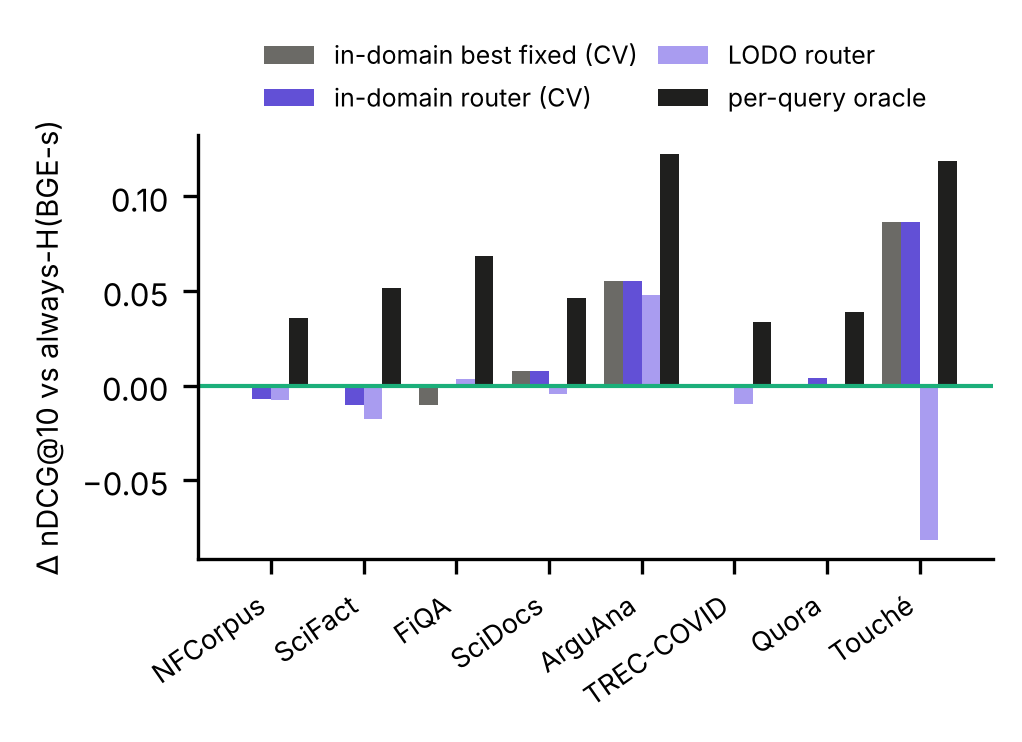
\includegraphics[width=0.92\columnwidth]{fig_indomain.png}
\caption{Gain over always-\Hy(BGE-s). The in-domain cross-validated router (purple) matches the in-domain best fixed system (grey); the LODO router (light purple) loses on Touch\'e; the per-query oracle (black) is out of reach.}
\label{fig:indomain}
\end{figure}

\subsection{Additional analysis}
\label{sec:additional}
The analyses in this subsection were not part of the original plan. They were added after the main results, and we report them separately for that reason. One of them, labelling by disagreement, was itself pre-registered before it was run.

\textbf{Removing the two smallest collections.} TREC-COVID (50 queries) and Touch\'e (49 queries) have the same weight as Quora (10,000 queries) in the macro average, so we repeat the main contrasts without them (Table~\ref{tab:sens}). Without Touch\'e, the BGE-s router is at $+0.002$ [$-0.003$, $+0.006$]; without Touch\'e and TREC-COVID, it is at $+0.004$ [$-0.001$, $+0.008$] ($p=0.06$). With BGE-b, the same exclusions give $+0.003$ [$-0.002$, $+0.008$] and $+0.006$ [$+0.001$, $+0.010$] ($p=0.01$); with Tier B signals, $+0.007$ [$+0.002$, $+0.012$]. On the six larger collections, a small routing gain with the stronger dense model is therefore possible. It only just exceeds the $+0.005$ threshold, and the router's loss on Touch\'e outweighs it in the headline. For the BGE-s text router, the exclusions give $-0.008$ and $-0.004$. For BM25 $-$ TF-IDF, the pooled difference without the two collections is $-0.005$ [$-0.039$, 0.029].

\begin{table}[t]
\centering
\caption{Additional analysis: macro $\Delta$ \ndcg{} on all 8 collections, without Touch\'e, and without Touch\'e and TREC-COVID. Stratified bootstrap CIs for rows 1--6 are in \texttt{numbers\_trace.md} in the code release (rows 1, 2 and 4 also in the text).}
\label{tab:sens}
\footnotesize
\setlength{\tabcolsep}{4pt}
\begin{tabular}{@{}lccc@{}}
\toprule
Contrast & All 8 & $-$Touch\'e & $-$Touch\'e $-$COVID \\
\midrule
Router $-$ \Hy{} (BGE-b) & $-0.013$ & $+0.003$ & $+0.006$ \\
Router $-$ \Hy{} (BGE-s) & $-0.009$ & $+0.002$ & $+0.004$ \\
Router $-$ \Hy{} (MiniLM) & $-0.008$ & $-0.010$ & $-0.007$ \\
Router $-$ \Hy{} (Tier B, BGE-b) & $-0.007$ & $+0.005$ & $+0.007$ \\
In-domain router $-$ \Hy{} (BGE-s) & $+0.017$ & $+0.007$ & $+0.008$ \\
CE(BM25) $-$ BM25 (sample) & $+0.025$ & $+0.052$ & $+0.037$ \\
Split-half choice (BGE-b) & $+0.015$ & $+0.009$ & $+0.012$ \\
Split-half choice (BGE-s) & $+0.018$ & $+0.008$ & $+0.010$ \\
$k{=}20$ choice (BGE-b) & $+0.012$ & $+0.006$ & $+0.008$ \\
$k{=}20$ choice (BGE-s) & $+0.014$ & $+0.004$ & $+0.005$ \\
$k{=}20$ choice (MiniLM) & $+0.008$ & $-0.003$ & $-0.003$ \\
\bottomrule
\end{tabular}
\end{table}

\textbf{How much of the oracle headroom is real.} Part of the per-query headroom is measurement noise. BM25 with and without stemming differs by only 0.0004 in macro \ndcg{} (and by at most 0.09 on single collections). An oracle choosing between these two per query already gains $+0.043$ over BM25. For BM25 vs.\ BM25+WordNet, the gain is $+0.013$. Against these reference points, the $+0.064$ three-way headroom is modest. The collection-level headroom, by contrast, holds on new queries: choosing the best fixed system on a random half of each collection and evaluating it on the other half (1,000 splits) gains $+0.0182$ for BGE-s, against $+0.0188$ in-sample (BGE-b: $+0.015$ vs.\ $+0.018$). The headroom is also concentrated. For BGE-s, the queries with an oracle gain above 0.2 are 2--27\% of all queries but carry 23--87\% of the headroom (BGE-b: 2--25\% and 18--88\%). On ArguAna, SciFact and Quora the median query has one relevant document, and queries with at most two relevant documents carry 83--100\% of the headroom. There, a per-query ``preference'' amounts to whether one document crosses rank 10.

\textbf{Choosing one system per collection from a few labels.} We choose one system (\B, \Dn{} or \Hy) per collection from $k$ random labelled queries and evaluate it on the remaining queries (1,000 draws; Fig.~\ref{fig:fewshot}). For BGE-s this gains $+0.004$, $+0.010$, $+0.014$ and $+0.016$ at $k=5,10,20,30$; for BGE-b, $+0.003$, $+0.009$, $+0.012$ and $+0.014$; for MiniLM, $-0.004$, $+0.005$, $+0.009$ and $+0.010$. These gains depend on Touch\'e. Without it, BGE-s gains $-0.006$, $0.000$, $+0.004$ and $+0.006$; BGE-b gains $-0.003$, $+0.002$, $+0.006$ and $+0.007$, mostly from ArguAna, where the dense model alone beats the hybrid; and MiniLM is negative for every $k\leq30$. Touch\'e, where BM25 is selected, is also the collection whose judgement pool favours BM25 (Section~\ref{sec:limits}).

\begin{figure}[t]
\centering
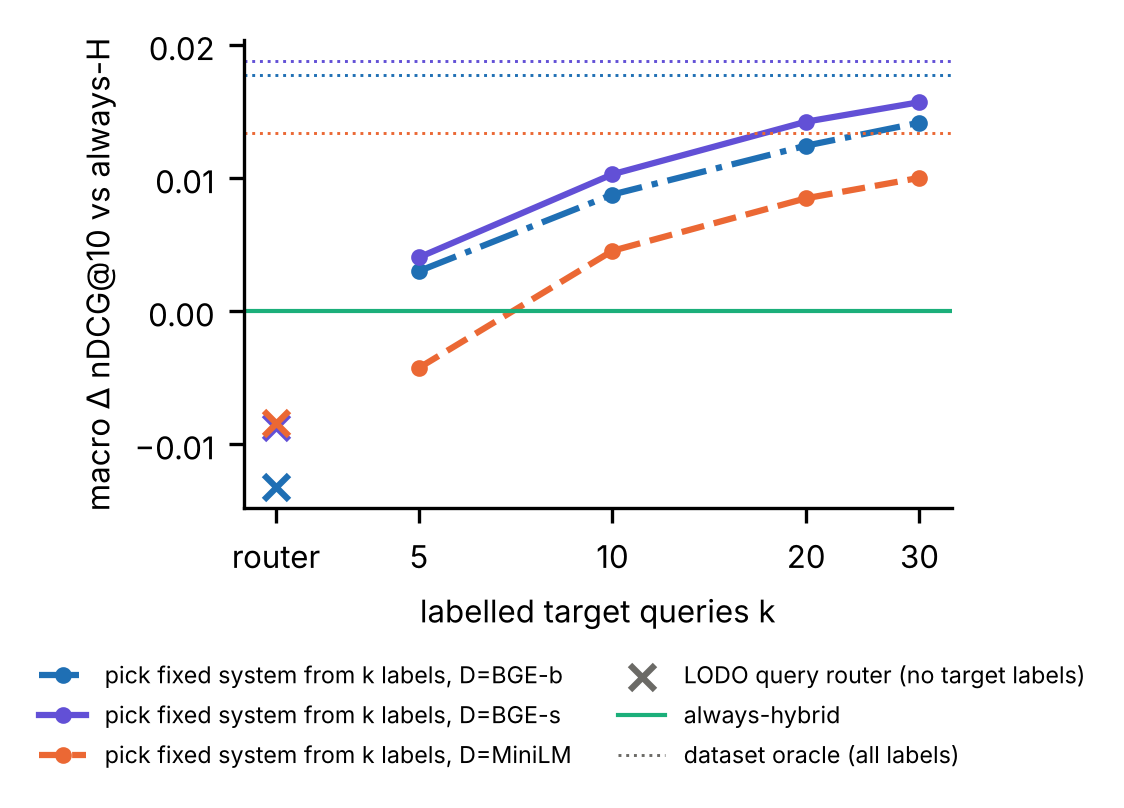
\includegraphics[width=0.85\columnwidth]{fig_fewshot.png}
\caption{Additional analysis: macro gain over always-\Hy{} when one fixed system is chosen per collection from $k$ labelled queries (mean of 1,000 draws). Crosses: LODO query routers. Most of the gain comes from Touch\'e (Table~\ref{tab:sens}).}
\label{fig:fewshot}
\end{figure}

\textbf{Tuning the hybrid weight from a few labels.} Choosing among only three systems is coarse. We therefore also choose the hybrid weight $\alpha\in\{0,0.1,\dots,1\}$ per collection from $k$ labelled queries (ties to 0.5; $\alpha=1$ is BM25 alone and $\alpha=0$ the dense model alone) and evaluate on the remaining queries (1,000 draws). We wrote this rule, with BGE-b at $k=20$ as the main contrast and ``a gain of at least $+0.005$ that remains without Touch\'e'' as the bar, before running it; the record is local and has no external timestamp. With BGE-b and $k=20$, the gain over \Hy$_{0.5}$ is $+0.021$ (2.5--97.5\% range over draws [$+0.011$, $+0.028$]); without Touch\'e it is $+0.013$, and without Touch\'e and ArguAna $+0.006$. At $k=10$ it is $+0.017$. This is larger than choosing among three systems ($+0.012$) and recovers 75.5\% of the hindsight per-collection optimum ($+0.027$). The selected weights favour the dense model ($\alpha=0.1$--0.4) everywhere except Touch\'e ($\alpha=0.9$). The gain holds for BGE-s ($+0.019$) and MiniLM ($+0.013$), but small losses remain on SciFact and Quora ($-0.002$ to $-0.003$ with BGE-b). The range covers only the choice of labelled queries, and part of the gain again comes from Touch\'e.

\textbf{Labelling by disagreement.} We pre-registered one refinement of the weight tuning: labelling the $k$ queries on which BM25 and BGE-b disagree most (lowest rank-biased overlap) instead of random ones. It did not help: $+0.002$ over random labelling at $k=20$ (pass bar $+0.003$), with 34\% of random draws doing at least as well, and losses with BGE-s and MiniLM.

\section{Discussion}
\label{sec:discussion}
\textbf{Why routing fails.} Three explanations fit the evidence.
\begin{itemize}
\item \emph{The signals measure difficulty, not preference.} They tell how hard a query is for every system. A router needs something else: which system is \emph{better} for this query. On that, the signals agree poorly with the truth ($\tau\leq0.12$). This matches the finding of Faggioli et al.\ that QPP fails where lexical and neural systems disagree~\cite{faggioli2023qpp}.
\item \emph{The per-query ``best system'' is noisy.} Many queries have only one or two relevant documents, so the winner often depends on a single document moving above or below rank 10. An oracle choosing between two near-identical versions of BM25 already gains $+0.043$.
\item \emph{The real differences are per collection.} Dense search wins clearly on ArguAna and BM25 on Touch\'e. A router trained on the other collections cannot learn a pattern that none of them shows, which is why it fails on Touch\'e. On Touch\'e, the dense results are less often judged than BM25's (judged@10 0.31 for BGE-b vs.\ 0.47), but BM25 still wins on judged-only lists (0.824 vs.\ 0.643). This agrees with Thakur et al., who find BM25 more effective on Touch\'e after removing unjudged short passages~\cite{thakur2024touche}.
\end{itemize}
Even when trained on the same collection, the router learns only the best fixed system for that collection, except on Quora, which has 8,000 training queries per fold.

\textbf{Practical guideline.} Use a hybrid of BM25 and a dense model. Without labelled queries, keep the 50/50 weight. With 10--20 labelled queries from the new collection, try weights from 0 to 1 on them and keep the best: in our additional analysis this adds $+0.017$ to $+0.021$ with BGE-b, mostly by giving the dense model more weight, and it identifies the collection where BM25 is better (Touch\'e). Do not copy BM25 settings tuned on other collections: this costs Touch\'e $-0.112$. Do not assume that a small cross-encoder improves a hybrid.

\textbf{Positioning.} Arabzadeh et al.\ train and test their per-query selector within one collection, MS~MARCO, with a fine-tuned BERT~\cite{arabzadeh2021predicting}. Our setting differs in data (across BEIR collections), router, metric and hybrid, so the two results are compatible: what does not transfer across collections is the router, not necessarily the signal. Our Quora fold, the one with many in-collection labels, shows a small learnable query-level signal. Khramtsova et al.\ find collection-level selection among dense retrievers ineffective without labels~\cite{khramtsova2023selecting}. We find the same at the query level. Our hybrid's exceptions (Touch\'e, ArguAna, Quora and SciDocs) largely coincide with those reported for the min-max hybrid of Kamalloo et al.~\cite{kamalloo2024resources}. Our result concerns cheap QPP signals and a small fine-tuned text encoder (Section~\ref{sec:method}); larger learned routers and large language models are not tested here. Mori et al.\ report query properties that change the BM25--dense gap in legal retrieval~\cite{mori2025assessing}. We find a label-based factor of this kind in all eight collections, but its label-free version fails. Their measures differ from ours, so the two results neither confirm nor contradict each other.

\section{Threats to Validity}
\label{sec:limits}
\begin{itemize}
\item \textbf{Power and weighting.} Eight collections can detect only $|\rho|\geq0.85$. The macro headline gives two collections of 49 and 50 queries a quarter of the weight, so we report results without them (Table~\ref{tab:sens}).
\item \textbf{Judgement pools.} On Touch\'e, only 47\% of BM25's top 10 is judged, and BM25's \ndcg{} rises from 0.444 to 0.824 on judged-only lists. The dense lists are judged less often still (judged@10 0.25--0.31). On NFCorpus, BM25's judged@100 is 0.186 vs.\ 0.078--0.087 for the dense models. On TREC-COVID, BGE-b and BM25 are judged equally often (judged@10 0.91), so pool bias does not explain the dense gain there. On Quora, judged-only \ndcg{} is 0.996--1.000 for every system and therefore uninformative. All Touch\'e statements carry this caveat.
\item \textbf{Model strength and router capacity.} Our dense models have 22--110M parameters. Moving from BGE-s to BGE-b raises every fixed system but leaves the routing conclusion unchanged; larger encoders (335M parameters and above) are untested. The CE results come from one small re-ranker on a query sample. Our routers are linear or tree models on hand-crafted signals, plus one 22M-parameter text encoder. On TREC-COVID and Touch\'e, the in-domain tree router is constant by construction (40-query folds, leaf size 50). The negative result is bounded to these choices.
\item \textbf{Configuration and statistics.} Flat and multifield BM25 differ by up to 0.077 on our collections. The router tests are not corrected across the 90 variant--configuration pairs; this does not weaken a negative claim, and we do not read the best pair as a win.
\item \textbf{Analyses added after the main results.} The analyses in Section~\ref{sec:additional} and the bootstrap confidence intervals were added after the main results. A single-annotator failure taxonomy from an earlier phase is omitted.
\end{itemize}

\section{Conclusion}
Across eight BEIR collections and three dense models, the best choice among BM25, dense and hybrid search can be predicted for a collection but not for a single query. A perfect per-query choice would gain $+0.065$ \ndcg{} over the hybrid with BGE-b, but an oracle over two near-identical BM25 versions already gains $+0.043$, so much of that headroom is noise. No router we built captures the rest, whether it uses standard QPP signals, list-agreement signals or the query text, predicts a weight, learns from a cross-encoder, or is trained on the same collection. These signals measure how hard a query is, which affects all systems alike. A fixed hybrid is the safe default. In our additional analysis, a few labelled queries, used to set its weight for the whole collection, improve on it ($+0.021$ with BGE-b).

\section*{Reproducibility}
The code covers indexing, retrieval, metrics, signals, routers, statistics and figures. It runs on 4 CPU cores; GPU encodings come from the provided Colab notebooks. The release also includes the per-query result files, the experiment logs with the planned tests, and scripts for every number (seed 42; $10^4$ permutations and resamples). All dense encodings were redone on a Colab GPU after the interim version of this paper. Locally encoded MiniLM rankings for five collections agree with them within 0.002 macro \ndcg{}; near-tied documents swap order for 72 queries. The agreement threshold was set to this tolerance before any downstream result was computed. The re-encoding changed the P1 result from $-0.0069$ (five collections) to $-0.0014$ (eight); no conclusion changed. The code, notebooks, per-query result files and the pre-registration texts are available at \url{https://github.com/aminah9945/ir-lexical-gap}.

\section*{Acknowledgment and Use of AI Tools}
The author thanks Dr.~Bilal for guidance and supervision, and her husband, Meherban, for support throughout this work. This work was carried out with extensive use of an AI assistant (Anthropic Claude, via Claude Code), under the direction of the author. The assistant:
\begin{itemize}
\item designed and ran the experiments and statistical analyses, and wrote the analysis code and the pre-declarations in the experiment logs;
\item searched and verified the literature;
\item drafted and revised this manuscript.
\end{itemize}
The author directed the work, ran the GPU notebooks in Google Colab, and takes full responsibility for the content.

\bibliographystyle{IEEEtran}
\bibliography{references}

\end{document}
